\documentclass[12pt]{article}
\usepackage{siunitx}
\usepackage{pgfplots}
\pgfplotsset{compat=1.18} % Or adjust depending on your TeX distribution
\usepackage[utf8]{inputenc}	% Para caracteres en español
\usepackage{amsmath,amsthm,amsfonts,amssymb,amscd}
\usepackage{multirow,booktabs}

\usepackage{mathabx}
\usepackage[table]{xcolor}
\usepackage{fullpage}
\usepackage{lastpage}
\usepackage{newtxmath}
\usepackage{newtxtext}
\usepackage{enumitem}
\usepackage{fancyhdr}
\usepackage{mathrsfs}
\usepackage{wrapfig}
\usepackage{setspace}
\usepackage{calc}
\usepackage{multicol}
\usepackage{cancel}
\usepackage[retainorgcmds]{IEEEtrantools}
\usepackage[margin=3cm]{geometry}
\usepackage{amsmath}
\newlength{\tabcont}
\setlength{\parindent}{0.0in}
\setlength{\parskip}{0.05in}
\usepackage{empheq}
\usepackage{framed}
\usepackage[most]{tcolorbox}
\usepackage{xcolor}
\colorlet{shadecolor}{orange!15}
\parindent 0in
\parskip 12pt
\geometry{margin=1in, headsep=0.25in}
\theoremstyle{definition}
\newtheorem{defn}{Definition}
\newtheorem{reg}{Rule}
\newtheorem{exer}{Exercise}
\newtheorem{note}{Note}
\newtheorem{theorem}{Theorem}
\setcounter{section}{0}
\usepackage{chngcntr}
\usepackage{hyperref}
\counterwithin*{equation}{section}
\counterwithin*{equation}{subsection}
\usetikzlibrary{angles,quotes,calc,positioning}
\usetikzlibrary{decorations.pathmorphing, patterns, calc}

\begin{document}

\section{Guía 1}

\begin{shaded}
    \textbf{(1)} Considerar la siguiente función de movimiento de un cuerpo que se desplaza en línea recta:
\[
x(t) = 1 \, [\tfrac{m}{s^2}] \, t^2 - 3 \, [\tfrac{m}{s}] \, t
\]
donde $x$ está dado en metros y $t$ en segundos.

\begin{itemize}
    \item[(a)] Graficar la función $x(t)$.
    \item[(b)] Determinar analíticamente en todos los casos y gráficamente en los siete primeros casos, los valores de velocidad media del móvil en los siguientes intervalos de tiempo (expresados en segundos): 

\begin{align*}
    &[-1, 5], \qquad [-1, 4], \qquad [-1, 1], \qquad [-1, -0.5], \\ 
    &[-1, -0.8], \qquad [-1, -0.9], [-1, -0.99], \\ 
    &[-1, -0.999], \; [-1, -0.9999].
\end{align*}

    \item[(c)] Sea $\Delta t_n = t_n - t_0$, con $t_0 = -1 \, s$, $t_1 = 5 \, s$, $t_2 = 4 \, s$, \ldots, $t_9 = -0.9999 \, s$. A medida que $t_n$ se hace más pequeño, ¿a qué valor se aproxima la velocidad media del móvil en el intervalo $[-1, -1 + \Delta t_n]$? ¿Cómo se interpreta geométricamente este resultado?
    \item[(d)] Encuentre la ecuación de la recta tangente a la función $x(t)$ en $t = -1 \, s$.
\end{itemize}
\end{shaded}

$(a)$ Graficar una función, primer año, no es necesario hacerlo. 

$(b)$ La velocidad media de un objeto en un intervalo de tiempo de longitud
$\Delta t$ se define como $\overline{v} = \Delta x / \Delta t$. Es fácil ver que
para la lista de intervalos que nos dieron, las velocidades medias son

\begin{equation*}
    1,\quad 0,\qquad -3,\qquad -4.5,\qquad -4.8,\qquad -4.9,\qquad -4.99,\qquad -4.999
\end{equation*}

$(c)$ Veamos que

\begin{align*}
    &\lim_{\Delta t \to 0} \frac{x(-1 + \Delta t) - x(-1)}{\Delta t} =
    \frac{dx}{dt}(-1)
\end{align*}

Es decir, el límite que nos interesa es la derivada evaluada en $-1$. Como 
$x'(t) = 2t - 3$, tenemos $2(-1) - 3 = -5$, lo cual coincide con lo que
observamos en $(b)$.

$(d)$ La recta tangente a $x(t)$ en un punto $(t_0, x(t_0))$ es la única recta
que atraviesa dicho punto y cuya
pendiente es la derivada de $x(t)$ en $t_0$. La pendiente en $t_0 = -1\text{s}$,
como ya vimos, es $a = -5$. Con lo cual sólo queda determinar $b \in \mathbb{R}$
tal que $\ell(t) = -5t + b$ satisfaga $\ell(-1) = x(-1) = 4$. Resolviendo: 

\begin{equation*}
    \ell(-1) = 4 \iff -5(-1) + b = 4 \iff b = -1
\end{equation*}

La recta deseada es $\ell(t) = -5t - 1$.

\pagebreak 

\begin{shaded}
    
\textbf{(2)} Considere la posición de un móvil que se desplaza en línea recta
bajo la ecuación $x(t)$ dibujada abajo, donde $\left[ x \right] = \text{m},
x(t=0) = -3\text{m}$.

$(a)$ Determinar la longitud total del camino recorrido en $I_0 = [-1, -0.8],
I_1=[-0.6, 0.6], I_2 = [-1, 1]$. 

$(b)$ Determinar la velocidad media en dichos intervalos.
 
$(c)$ Determinar gráficamente la velocidad instantánea del móvil en los
siguientes instantes: $t = 0, t  = 0.8$.

$(d)$ Determinar aproximadamente para qué valores de $t$ el móvil se encuentra a
$1$m de distanca de la posición que tiene en $t = 0$.

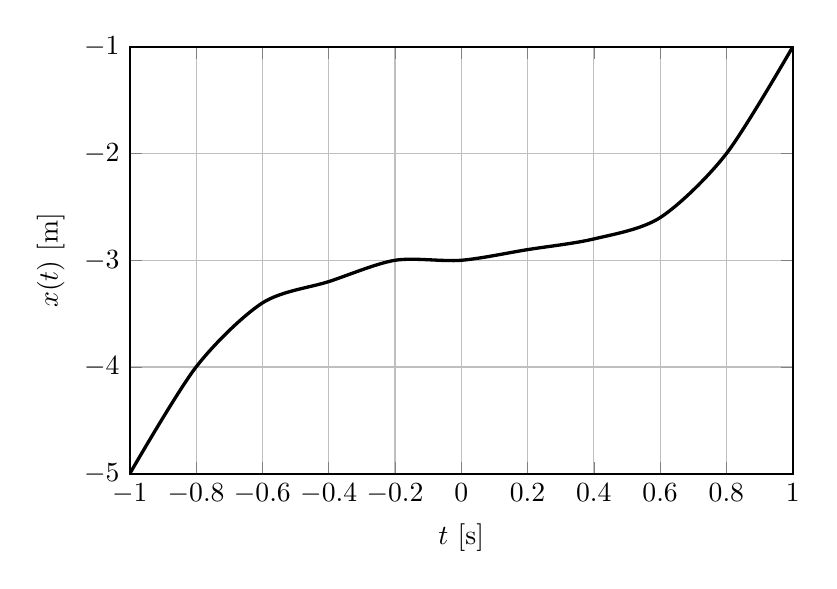
\begin{tikzpicture}
  \begin{axis}[
    width=10cm,
    height=7cm,
    grid=both,
    xlabel={$t$ [s]},
    ylabel={$x(t)$ [m]},
    thick,
    xmin=-1, xmax=1,
    ymin=-5, ymax=-1,
    ]
    % Example plot points (replace with your data or function)
    \addplot[black, very thick, smooth] coordinates {
      (-1.0,-5.0)
      (-0.8,-4.0)
      (-0.6,-3.4)
      (-0.4,-3.2)
      (-0.2,-3.0)
      (0.0,-3.0)
      (0.2,-2.9)
      (0.4,-2.8)
      (0.6,-2.6)
      (0.8,-2.0)
      (1.0,-1.0)
    };
  \end{axis}
\end{tikzpicture}
\end{shaded}

$(a)$ En el intervalo de tiempo $I_0$, el móvil se movió de la posición
$-5\text{m}$ a $-4\text{m}$, i.e. recorrió un metro. Etc. 

$(b)$ Ya sabemos hacer esto: $\overline{v} = \Delta x / \Delta t$. Etc. 

$(c)$ La velocidad instantánea en un punto $t_0$ se calcula gráficamente
dibujando la recta tangente a $x(t_0)$ y determinando la pendiente de dicha
recta. 

$(d)$ Gráficamente, se ve que se da en $t = 0.8, t = -0.8$.

\pagebreak 

\begin{shaded}
    \textbf{(5)} Sea $x(t) = -5t^2 + 17t + 3$ la función de posición de una
    partícula con $\left[ x \right] = \text{m}, \left[ t \right] = \text{s} $. 

    $(a)$ Determinar la posición de la partícula en $t =1,2,3\text{s}$.

    $(b)$ Determinar el tiempo en que la partícula retorna al origen.

    $(c)$ Obtenga $v(t)$ y determine la velocidad instantánea en
    $t=1,2,3\text{s}$, cuándo la velocidad es nula, y cuál es la velocidad de la
    partícula cuando pasa por el origen. 

    $(d)$ Grafique $x(t), v(t), a(t)$.
\end{shaded}

$(a)$ Una pavada, evaluar $x(t)$ en esos valores. 

$(b)$ La partícula retorna al origen siempre que $x(t) = 0$, con soluciones 

\begin{equation*}
    t = \frac{-17 \pm \sqrt{17^2 - 4 \cdot (-5) \cdot 3} }{-10} \iff t \in
    \left\{ -0.16815416922, 3.56815416923 \right\} 
\end{equation*}

Pero el tiempo no puede ser positivo, con lo cual la única solución que
consideramos es $t_0 \approx 3.568$.

$(c)$ $v(t) = x'(t) = -10t + 17$. La velocidad en los tiempos dados se obtiene
evaluando la función (trivial). La velocidada es nula si y solo si 

\begin{equation*}
    v(t) = 0 \iff t = \frac{17}{10} \iff t = 1.7
\end{equation*}

La velocidad al pasar por el origen es $v(t_0) \approx v(3.568) = -18.68$.

$(d)$ $a(t) = v'(t) = -10$ es una función constante. $v(t)$ es lineal y fácil de
calcular. De $x(t)$ ya conocemos las raíces, sabemos que tiene "alas" hacia
abajo (pues el coeficiente $a$ de la cuadrática es negativo), y que el máximo es
el punto medio entre las raíces, i.e. 

\begin{equation*}
    t_{\text{max}} =  \frac{ -0.16815416922 + 3.56815416923 }{2} = \frac{3.4}{2}
    = 1.7
\end{equation*}

Esto es suficiente para hacer un gráfico aproximado. Podemos agregar que $x(0) =
3$ si queremos ser más bonitos aún.

\pagebreak 

\begin{shaded}
    \textbf{6.} La figura muestra la velocidad de un móvil en función del tiempo:

\begin{center}
\begin{tikzpicture}
\begin{axis}[
    axis lines=middle,
    xlabel={$t \; [s]$},
    ylabel={$v \; [km/s]$},
    xmin=0, xmax=16,
    ymin=0, ymax=50,
    xtick={0,2,6,9,15},
    ytick={0,20,44},
    width=12cm,
    height=7cm,
    samples=200,
    domain=0:15,
]
\addplot[thick,black] coordinates {
    (0,20) (6,20) (9,44) (15,0)
};
\end{axis}
\end{tikzpicture}
\end{center}

\begin{enumerate}
    \item[(a)] Determine la aceleración instantánea del móvil para $t=3\,s$ y $t=11\,s$.
    \item[(b)] Calcule la distancia recorrida por el móvil en los intervalos de tiempo $t=[0,5]\,s$, $t=[0,9]\,s$ y $t=[0,15]\,s$.
    \item[(c)] Conociendo que $x(t=6\,s)=0\,m$, encuentre la posición del móvil en $t=0\,s$.
    \item[(d)] Dé una expresión de la posición del móvil válida para todo $t$.
    \item[(e)] Grafique $x(t)$, $v(t)$ y $a(t)$.
\end{enumerate}
\end{shaded}

$(a)$ Del gráfico obtenemos que 

\begin{equation*}
    v(t) = \begin{cases}
        20 & 0 \leq t < 6\\ 
        \ell_1(t) &6 \leq t < 9 \\ 
        \ell_2(t) &9\leq t \leq 15
    \end{cases}
\end{equation*}

donde $\ell_1, \ell_2$ son funciones lineales a determinar. Sabemos que
$\ell_1(6) = 20, \ell_1(9) = 44$, lo cual es suficiente para determinar la
función. La pendiente es

\begin{equation*}
    a_1 = \frac{\Delta \ell_1}{\Delta t} = \frac{44 - 20}{9 - 6} = 8
\end{equation*}

Como $\ell_1(6) = 20$, necesitamos $8\cdot 6 + b_1 = 20 \iff b_1 = -28$. 

$\therefore $ $\ell_1(t) = 8t - 28$.

De manera análoga se determina que $\ell_2(t) = - \frac{22}{3}t + 110$.

Sabiendo $v(t)$, determinamos la aceleración como 

\begin{equation*}
    a(t) = v'(t) = \begin{cases}
        0 & 0 \leq t < 6 \\ 
        8 & 6 \leq t < 9 \\ 
        -\frac{22}{3} & 9 \leq t \leq 15
    \end{cases}
\end{equation*}

lo cual es suficiente para calcular la aceleración instantánea en los puntos de
interés.

$(b)$ La distancia recorrida por un móvil con función de velocidad $v(t)$ en un
intervalo de tiempo $I$ es 

\begin{equation*}
    \int_I \left| v(t) \right| ~ dt
\end{equation*}

Para un intervalo general $I = [a, b]$, usando el hecho de que $v(t) > 0
\Rightarrow \left| v(t) \right| = v(t)$,

\begin{equation}
    \int_I \left| v(t) \right| ~ dt 
    &= x(b) - x(a)
\end{equation}

pues $x(t)$ es la primitiva de $v(t)$. Pero 

\begin{align*}
    x(t) 
    &= \int v(t) ~ dt \\ 
    &=\begin{cases}
        20t + \varphi_1 & 0 \leq t < 6 \\ 
        4t^2 - 28t + \varphi_2 & 6 \leq t < 9 \\ 
        -\frac{22}{6}t^2 + 110t + \varphi_3 & 9 \leq t \leq 15
    \end{cases}
\end{align*}

para algunas constantes $\varphi_1,  \varphi_2, \varphi_3 \in \mathbb{R}$.
Dichas constantes dependen del sistema de coordenadas elegido para la función de
posición, pero además deben satisfacer las restricciones de continuidad. Sabemos
que $x(6) = 0$ por el enunciado $(c)$. Entonces $x(6) = 20t + \varphi_1 = 0 \iff
\varphi_1 = -120$. Para satisfacer continuidad, necesitamos 

\begin{equation*}
    20(6) - 120 = 4(6^2) - 28(6) + \varphi_2 \iff \varphi_2 = 24
\end{equation*}

De manera análoga se obtiene $\varphi_3= -597$. Por lo tanto, 

\begin{equation*}
    x(t) = \begin{cases}
        20t - 120 & 0 \leq t < 6 \\ 
        4t^2 -28t  + 24 & 6 \leq t < 9 \\ 
        -\frac{22}{6}t^2 + 110t -597 & 9 \leq t \leq 15
    \end{cases}
\end{equation*}

Usando la ecuación $(1)$, la distancia recorrida en $I_0 = [0, 5]$ será 

\begin{equation*}
    x(5) - x(0) = -20 + 120 = 100
\end{equation*}

(en kilómetros). Para $I_1 = [0, 9]$ será 

\begin{equation*}
    \int_0^6 v(t) ~ dt + \int_6^9 v(t) ~ dt = \left[ x(6) - x(0) \right] +
    \left[ x(9) - x(6) \right] = \text{etc.}
\end{equation*}

$(d)$ Ya lo hicimos al hallar $x(t)$. 

$(e)$ Etc.

\pagebreak 

\begin{shaded}
    \textbf{(7)} Un camión y un auto parten en el instante $t=0$, el auto
    estando cierta distancia $\Delta x$ tras el camión. El camión  tiene una
    aceleración $a_{\text{truck}} = 1.2\text{m/s}^2$, el auto una aceleración
    $a_{\text{car}} = 1.8\text{m/s}^2$. El auto alcanza al camión cuando éste ha
    recorrido 45m. 

    $(a)$ Determinar el tiempo $t_*$ que tarda el auto en alcanzar al camión.

    $(b)$ Determinar $\Delta x$. 

    $(c)$ Determinar $v_{\text{car}}(t_*), v_{\text{truck}}(t_*)$.

    $(d)$ Graficar posición, velocidad y aceleración de ambos.
\end{shaded}

$(a)$ Sabiendo las aceleraciones, podemos determinar las velocidades y con ellas
las posiciones. En particular, 

\begin{align*}
    &v_{\text{car}}(t) = 1.8 t \text{ m/s} + \alpha_1 \text{ m/s}, \qquad x_{\text{car}}(t) =
    0.9t^2 + \alpha_1 t \text{ m} + \alpha_2\text{ m}\\ 
    &v_{\text{truck}}(t) = 1.2\text{ m/s} + \beta_1\text{ m/s},\qquad x_{\text{truck}}(t) =
    0.6t^2\text{ m} + \beta_1 t \text{ m} + \beta_2 \text{ m}
\end{align*}

con $\alpha_i, \beta_i \in \mathbb{R}$ para $i=1,2$. Ambos vehículos
parten en el instante $t=0$, así que en dicho instante sus velocidades son
nulas:

\begin{equation*}
    v_{\text{car}}(t=0) = 0 \Rightarrow \alpha_1 =0, \qquad
    v_{\text{truck}}(t=0) = 0 \Rightarrow \beta_1 = 0
\end{equation*}

Si definimos el origen de nuestro sistema como el punto de partida del auto,

\begin{align*}
    x_{\text{car}}(t=0) = 0 \Rightarrow  \alpha_2 = 0, \qquad
    x_{\text{truck}}(t=0) =  \Delta x \Rightarrow \beta_2 = \Delta x
\end{align*}

Por lo tanto,

\begin{align*}
    &v_{\text{car}}(t) = 1.8 t \text{ m/s}, \qquad x_{\text{car}}(t) =
    0.9t^2, \\
    &v_{\text{truck}}(t) = 1.2\text{ m/s}, \qquad x_{\text{truck}}(t) =
    0.6t^2\text{ m} + \Delta x\text{ m}
\end{align*}

El instante $t_*$ es el instante en que el camión ha recorrido 45m:


\begin{align*}
    \int_0^{t_*} v_{\text{truck}}(t) ~ dt = 45 \iff 
    &x_{\text{truck}}(t_*) - x_{\text{truck}}(0) = 45 \\ 
    \iff ~ ~ ~ 
    &0.6t_*^2 + \Delta x - \Delta x = 45 \\ 
    \iff  ~ ~  ~ 
    &0.6t_*^2 = 45 \\ 
    \iff ~ ~ ~ 
    &t_*^2 = 75 \\ 
    \iff ~ ~ ~ 
    &t_* = 5\sqrt_*{3}  
\end{align*}

$(b)$ Sabemos que $x_{\text{car}}(t_*) = x_{\text{truck}}(t_*)$, con lo cual
obtenemos 

\begin{equation*}
    0.9(5\sqrt{3} )^2 = 0.6(5\sqrt{3} )^2 + \Delta x \iff \Delta x = 22.5
\end{equation*}

$(c)$ Una pavada. 

$(d)$ Una pavada.

\pagebreak 

\begin{shaded}
    \textbf{(8)} Un automóvil se desplaza por una carretera que es paralela a la vía de un tren. El automóvil se detiene ante un semáforo que está con luz roja en el mismo instante que pasa un tren con una velocidad constante de $12.0 \, \mathrm{m/s}$. El automóvil permanece detenido durante $6.0 \, \mathrm{s}$ y luego parte con una aceleración constante de $2.0 \, \mathrm{m/s^2}$.  

Determine:
\begin{enumerate}[(a)]
    \item El tiempo que emplea el automóvil en alcanzar al tren, medido desde el instante en que se detuvo ante el semáforo.
    \item La distancia que recorrió el automóvil desde el semáforo hasta que alcanzó al tren.
    \item La velocidad del automóvil en el instante que alcanza al tren.
\end{enumerate}
\end{shaded}

$(1)$ Sea $t = 0$ el tiempo en que el auto se detiene en el semáforo, y $x(0)$
la posición del semáforo. Sabemos que para $t \geq 6$,

\begin{equation*}
    v_{\text{car}}(t) = 2t \text{ m/s} + \alpha_1, \qquad x_{\text{car}}(t) =
    t^2 \text{ m} + \alpha_1 t + \alpha_2
\end{equation*}

siendo ambas funciones constanatemente nulas para $0 \leq t < 6$.

Como la velocidad en el instante $t=6$ es nula, $v_{\text{car}}(6) = 0 \iff 12 +
\alpha_1 = 0 \iff \alpha_1 = -12$. Como la posición en el instante 6 es nula,
$6^2 -12(6) + \alpha_2 = 0 \iff \alpha_2 = 36$.

\begin{equation*}
    \therefore \qquad v_{\text{car}}(t) = 2t \text{ m/s} - 12\text{ m/s}, \qquad x_{\text{car}}(t) =
    t^2 \text{ m} -12t \text{ m} + 36\text{ m}
\end{equation*}

para $t \geq 6$. De manera análoga, para todo $t \geq 0$,

\begin{equation*}
    x_{\text{train}}(t) = 12t  \text{ m}
\end{equation*}

donde la constante de integración debe ser cero para satisfacer que la posición
del tren en el instante inicial es nula.

El tiempo $t_* > 6$ en que el auto alcanza al tren satisface 

\begin{align*}
x_{\text{train}}(t_*)
= x_{\text{car}}(t_*) 
\iff 
&12t_* = t_*^2 -12 t_* + 36\\ 
\iff
&t_*^2 -24t_* + 36 = 0
\end{align*}

con soluciones 

\begin{equation*}
    t_* = \frac{24 \pm \sqrt{24^2 -4 (36)} }{2} \iff t_* \in \left\{
    1.60769515459, 22.3923048454 \right\} 
\end{equation*}

La solución $t_* \approx 1.608$ no debe considerarse y por ende $t_* \approx
22.392$.

$(2)$ La distancia recorrida por el automóvil desde el semáforo hasta que
alcanzó el tren es dada por 

\begin{align*}
    \int_{t=0\text{s}}^{t=t_*\text{s}} \left| v_{\text{car}}(t) \right| ~ dt 
    &= \int_{t=6\text{s}}^{t={t_* \text{s}}} \left| v(t) \right| ~dt \\
    &= \int_{t=6\text{s}}^{t={t_* \text{s}}}  v(t) ~dt \\ 
    &=x(t_*) - x(6)\\ 
    &=x(t_*)
\end{align*}

donde el valor absoluto desaparece puesto que en $t \geq 6$ la función integrada
es claramente mayor o igual a cero. Usando la aproximación $t_* \approx 22.392$,
se obtiene $x(t_*) \approx 268.697 \text{ m}$.

$(c)$ Una pavada: evaluar $v_{\text{car}}(t_*)$.

\pagebreak 

\begin{shaded}
    \textbf{(11)} El movimiento en el plano de una partícula es dado por 
    $x(t) = at^2$ e $y(t) = bt^3$ con $a = 3 \text{m/s}^2, b = 2\text{m/s}^3$.

    $(a)$ Hallar la trayectoria de la particula. 

    $(b)$ Calcular su aceleración en $t = 12$s. 

    $(c)$ Calcular el ángulo entre los vectores velocidad y aceleración en dicho
    instante. 

    $(d)$ Determinar el instante $t_1$ en que la aceleración es paralela a la
    recta $y = x$ y el instante $t_2$ en que la velocidad lo es. 

    $(e)$ Determinar la velocidad media entre los dos instantes calculados en
    $(d)$.
\end{shaded}


$(a)$ La trayectoria es el conjunto de puntos 

\begin{align*}
    S 
    &= \left\{ \left( x(t),  y(t) \right) : t \in \mathbb{R}  \right\} \\ 
    &= \left\{ (at^2, bt^3) : t \in \mathbb{R}\right\} 
\end{align*}

Dado un punto $p_0 = (x, y)$ arbitrario de la trayectoria, se satisface que 

\begin{equation*}
    x = at^2, \qquad y = bt^3
\end{equation*}

Tomemos $t \geq 0$. De la primera ecuación deducimos $t =
\sqrt{\frac{x}{a}} $. De la segunda ecuación deducimos 

\begin{equation*}
    y = bt^3 = b \left( \frac{x}{a}
    \right)^{\frac{3}{2}}
\end{equation*}

Por lo tanto, para todo $t \geq 0$, la función 

\begin{equation*}
    \tau(x) = b\left( \frac{x}{a} \right)^{\frac{3}{2}}
\end{equation*}

describe la trayectoria del móvil.

$(b)$ La velocidad y aceleración del móvil es dada por

\begin{equation*}
    v_x(t) = 2at, \qquad a_x(t) = 2a, \qquad \qquad v_y(t) = 3bt^2, \qquad
    a_y(t) = 6bt
\end{equation*}

o más rigurosamente 

\begin{equation*}
    v(t) = 6t \hat{i} + 6t^2 \hat{j}, \qquad a(t) = 6 \hat{i} + 12t \hat{j}
\end{equation*}

La aceleración en $t = 12$ es trivial: evaluar $a(t)$ en dicho valor.


$(c)$ A calcularla nomás: 

\begin{equation*}
    v(12) = 72 \hat{i} + 864 \hat{j}, \qquad \qquad
    a(12) =  6 \hat{i} + 144 \hat{j}
\end{equation*}

donde la unidad de la coordenada $x$ está en $\text{m/s}^2$, y la de $y$ en
$\text{m/s}^3$. Recordemos que el producto punto entre dos vectores se define 
como

\begin{equation*}
    \vec{w} \cdot \vec{u} = uw \cos \theta
\end{equation*}

con $\cos \theta$ el ángulo entre ellos, pero que además satisface que 
$\vec{w} \cdot \vec{u} = \vec{w}_x \vec{u}_x + \vec{w}_y \vec{u}_y$. Por ende,
el producto cruz de los vectores de aceleración y posición satisface 

\begin{align*}
    72(6) + 864(144) = \left| v(12) \right| \left| a(12) \right|
    \cos \theta
\end{align*}

Las magnitudes de ambos vectores son 

\begin{equation*}
    \left| v(12) \right| = 866.995, \qquad \left| a(12)
    \right| = 144.125
\end{equation*}

Sustituyendo con el resultado de las operaciones y dividiendo por el producto de
las magnitudes, obtenemos

\begin{equation*}
    0.99827265479 = \cos \theta \iff \theta = 1.51201125\text{rad}
\end{equation*}

$(d)$ Queremos saber el instante $t_1$ en que el ángulo $\varphi$ entre la
aceleración y la recta $y = x$ es nulo, i.e. el momento en que el ángulo entre
la aceleración y el eje $x$ es $\frac{\pi}{4}$. Hay dos formas de resolver esto.
La más simple es ver que el vector tiene dicho ángulo si y solo si la componente
$x$ es igual a la componente $y$, y planteando al ecuación 

\begin{equation*}
    a_x(t_1) = a_y(t_1) \iff 6 = 12t_1 \iff t_1 = 1 / 2
\end{equation*}

Sólo para tener en cuenta que nos podrían haber pedido un ángulo $\varphi$ menos
obvio respecto al eje $x$, la forma general (pero más densa) de calcular esto
es planteando la ecuación:

\begin{align*}
    &\frac{ \vec{a}(t_1) \cdot \hat{i} }{\left| \vec{a}(t_1) \right| \left|
    \hat{i} \right| } = \cos \varphi \\
    \iff ~ ~ ~ 
    &\frac{a_x(t_1)}{\left| \vec{a}(t_1)
\right| } = \cos(\frac{\pi}{4}) \\ 
\iff ~ ~ ~ 
    &\frac{6}{\sqrt{6^2 + 12^2t_1^2} } = 
\frac{ \sqrt{2}  }{2} \\ 
\iff ~ ~ ~ 
    &\frac{ 36 }{36 + 144t_1^2} = \frac{1}{2}\\ 
    \iff ~ ~ ~ 
    &72 = 36 + 144t_1^2\\
    \iff ~ ~ ~ 
    &144t_1^2 -36 = 0 \\ 
    \iff ~ ~ ~ 
    &36\left( 4t_1^2 - 1 \right) =0 \\ 
    \iff ~ ~ ~ 
    &4t_1^2 - 1 = 0\\
    \iff ~ ~ ~ 
    &4t_1^2 = 1\\
    \iff ~ ~ ~ 
    &t_1^2 = \frac{1}{4}
\end{align*}

Como $t > 0$ esto da una única solución $t_1 = 1 / 2$. Para la velocidad hacemos
solo la forma simple, viendo que 

\begin{equation*}
    v_x(t_2) = v_y(t_2) \iff 6t_2 = 6t_2^2 \iff t_2 = t_2^2 \iff t = 1
\end{equation*}

(pues $t > 0$).  

$(e)$ La velocidad media entre los dos instantes es 


\begin{equation*}
    \Delta \vec{x} / \Delta t = \frac{(3 * 1^2 - 3*( 0.5^2 ), 2*1^3 -
    2*(0.5^2)}{0.5} = \frac{(2.25, 1.75)}{0.5} = (4.5, 3.5)\text{m/s}
\end{equation*}

\pagebreak 

\section{Guía 2}

\begin{shaded}
    \textbf{(1)} La siguiente figura muestra una masa $A$ de $100 \,\text{kg}$, apoyada sobre la superficie de un plano inclinado. 
No existe rozamiento entre la masa $A$ y la superficie del plano inclinado. 
La cuerda $AB$ es paralela al plano en que se apoya $A$, en tanto que la cuerda $AC$ está horizontal. 
Calcular:
\begin{enumerate}
  \item el peso del bloque $P$ sabiendo que el sistema está en equilibrio,
  \item la reacción del plano sobre el bloque $A$.
\end{enumerate}

\begin{center}
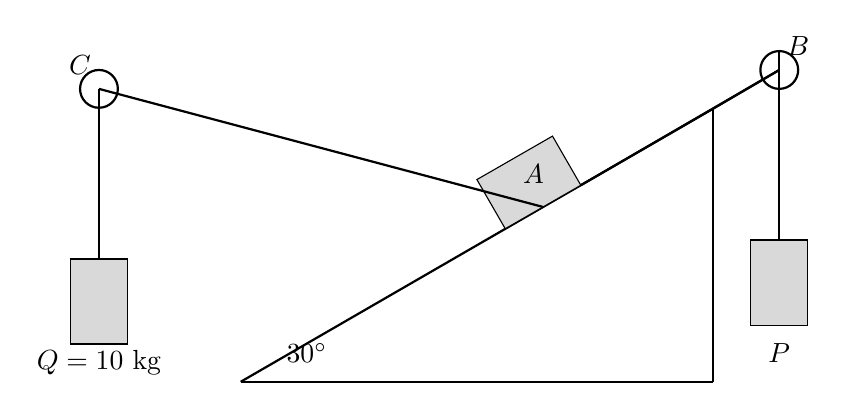
\begin{tikzpicture}[scale=1.2]
  % Plano inclinado
  \draw[thick] (0,0) -- (5,0);
  \draw[thick] (0,0) -- (5,2.89); % inclinación 30°
  \draw[thick] (5,0) -- (5,2.89);
  \node at (0.7,0.3) {$30^\circ$};

  % Bloque A
  \draw[fill=gray!30] (2.8,1.62) -- ++(0.8,0.46) -- ++(-0.3,0.52) -- ++(-0.8,-0.46) -- cycle;
  \node at (3.1,2.2) {$A$};

  % Polea B
  \draw[thick] (5,2.89) -- (5.7,3.3);
  \draw[thick] (5.7,3.3) circle (0.2);
  \node at (5.9,3.55) {$B$};

  % Polea C
  \draw[thick] (-1.5,2.4) -- (-1.5,3.1);
  \draw[thick] (-1.5,3.1) circle (0.2);
  \node at (-1.7,3.35) {$C$};

  % Cuerdas
  \draw[thick] (3.6,2.08) -- (5.7,3.3); % A-B
  \draw[thick] (3.2,1.85) -- (-1.5,3.1); % A-C
  \draw[thick] (5.7,3.5) -- (5.7,1.5); % cuerda a P
  \draw[thick] (-1.5,2.9) -- (-1.5,1.3); % cuerda a Q

  % Bloques P y Q
  \draw[fill=gray!30] (5.4,1.5) rectangle (6,0.6);
  \node at (5.7,0.3) {$P$};

  \draw[fill=gray!30] (-1.8,1.3) rectangle (-1.2,0.4);
  \node at (-1.5,0.2) {$Q=10$ kg};
\end{tikzpicture}
\end{center}

(El gráfico es sólo esquemático: la cuerda AB es horizontal!)
\end{shaded}

$(1)$ Definamos un nuevo sistema de coordenadas, con un vector unitario paralelo
a la superficie y otro perpendicular a la superficie: 

\begin{equation*}
    \hat{p} = (\cos \theta, \sin \theta), \qquad \hat{n} = (-\sin \theta, \cos
    \theta)
\end{equation*}

(por $\hat{p}$aralela y $\hat{n}$ormal). Recordemos que la proyección escalar de
un vector $\vec{v}$ sobre un vector $\vec{w}$ se define como $\vec{v} \cdot
\vec{w}$.

El sistema está en equilibrio. Por ende, las fuerzas que mueven la masa $A$
hacia arriba y hacia abajo de la superficie suman cero (se equilibran). Dichas
fuerzas son 

\begin{equation*}
    \vec{G} = -m_A g \hat{j}, \qquad \vec{F_Q} = -m_Qg \hat{i}, \qquad \vec{F_P}
    = m_P g \hat{p}
\end{equation*}

Por ende,

\begin{equation}
    G_{\parallel} + F_{Q ~ \parallel} + F_{P ~ \parallel} = 0
\end{equation}

donde el sufijo $\parallel$ indica "el componenete paralelo a la superficie" de
la fuerza y $\vec{G}$ es la fuerza de la gravedad. Ya dijimos que dicho
componente será el producto punto entre cada vector y $\hat{p}$. 


\small
\begin{quote}

\textbf{Nota.} Si un vector ya es paralelo a cierto vector unidad, como
$\vec{F_P}$ es paralelo a $\hat{p}$, la proyección de dicho vector sobre el
unitario es simplemente la magnitud del vector. Es decir, $F_{P ~ \parallel} =
\vec{F_P} \cdot \hat{p} = F_P$. (Ver nota al final para una demostración.) 
\end{quote}
\normalsize

Obtenemos entonces que la ecuación $(1)$ resulta:


\begin{equation}
    -m_A g \sin \theta  + (-m_Q g)\cos\theta + m_P g = 0
\end{equation}

de lo cual se sigue que 

\begin{equation*}
    m_P = m_A \sin \theta + m_Q \cos \theta = 100\text{kg}\frac{1}{2} +
    10\text{kg} \frac{\sqrt{3} }{2} = 58.6602540378\text{kg}
\end{equation*}



$(2)$ Como no hay fricción, la reacción del plano sobre el bloque es dada
estrictamente por la fuerza normal. Dicha fuerza es paralela al vector unitario
$\hat{n}$, i.e. es perpendicular a la superficie. Su magnitud debe
contraarrestar la de todas las fuerzas que actúan en dirección perpendicular a
la superficie. Dichas fuerzas son la gravedad y la fuerza de la polea estirada
por $Q$, con componentes perpendiculares a la superficie dados por:

\begin{align*}
    &G_{\perp} = \vec{G} \cdot \vec{n} = -m_A g \cos \theta = - ( 100\text{kg}
    \cdot
    \sqrt{3}/2 \cdot
    \cdot 9.8\text{m/s}^2) = -848.704895709\text{N}\\
    &F_{Q \perp} = \vec{F_Q} \cdot \vec{n} = (-m_Q g)(- \sin \theta) =
    10\text{kg} \cdot 1 / 2 \cdot 9.8\text{m/s}^2 =  49\text{N}
\end{align*}

La suma de ambas componentes nos da $-848.704895709\text{N} + 49\text{N} =
-799.704895709$, lo cual quiere decir que $N \approx 800\text{N}$ es la reacción
del plano.

\pagebreak 

\begin{shaded}
    \textbf{(2)} Un cuerpo de masa $m = 10$kg está apoyado en una superficie
    horizontal sin rozamiento. Una persona tira del bloque con una soga fija al
    bloque en dirección horizontal con una fuerza de 20N. Calcular la
    aceleración del bloque suponiendo despreciable la masa de la soga.
\end{shaded}

Como el movimiento es horizontal, $\vec{a} = a \hat{i}$ y solo basta determinar
$a$. Por la segunda ley de Newton, $F = ma$, de lo cual se sigue que 
$20\text{N}/10\text{kg} = a$, es decir $a = 2\text{m/s}^2$.

\pagebreak 

\begin{shaded}
    \textbf{(4)} Un bloque $A$ de masa $m_A = 8$kg descansa sobre un plano
    inclinado con ángulo $\alpha = \ang{37}$, unido con una cuerda y una polea
    sin rozamiento a un bloque $B$ de masa $m_B = \text{4}$kg. Determina la
    aceleración $\vec{a}$ de las masas y la tensión de la cuerda cuando se deja
    al sistema evolucionar libremente. Realice un diagrama de cuerpo aislado.
\end{shaded}

Sean 

\begin{equation*}
    \hat{p} = (\cos \alpha, \sin \alpha),\qquad \hat{n} = (-\sin \alpha, \cos\alpha)
\end{equation*}

los vectores unitarios de un sistema de coordenadas con ejes paralelo
($\hat{p}$) y perpendicular ($\hat{n}$) al plano inclinado.

$A$ se mueve paralelo al plano. Luego $\vec{a_A} = a_A \hat{p}$ y solo queda
determinar $a_A$. $B$ se mueve verticalmente. Luego $\vec{a_B} = a_B \hat{j}$ y
solo queda determinar $a_2$. Por la segunda ley de Newton, 

\begin{equation*}
    m_A a_{A} = G_{A ~ \parallel} + T, \qquad m_B a_B = G_B + T 
\end{equation*}

con el sufijo $\parallel$ indicando el componente de una fuerza paralelo al
plano inclinado. Es claro que $a_A = -a_B$. Además, de la segunda ecuación
arriba podemos tomar $T = m_B a_B - G_B$. Sustituyendo en la primera expresión, 

\begin{align*}
    m_Aa_A 
    &= G_A_{\parallel} + \left( m_B a_B - G_B \right)  \\ 
    &= G_{A \parallel} - m_Ba_A - G_B \\ 
\end{align*}

con lo cual obtenemos una ecuación con única incógnita $a_A$. Resolviendo: 

\begin{align*}
    a_A 
    &= \frac{ G_{A ~ \parallel}- G_B }{m_A + m_B}\\ 
    &= \frac{( \vec{G_A} \cdot \hat{p} ) - (- m_Bg )}{12\text{kg}}\\
    &= \frac{( -m_A g \sin \alpha) + m_Bg}{12\text{kg}}\\ 
    &=\frac{-8\text{kg}\cdot 9.8 \text{m/s}^2\cdot 0.602) + 4\text{kg}\cdot 9.8
    \text{m/s}^2}{12\text{kg}} \\ 
    &=\frac{(-8\cdot 9.8 \text{m/s}^2\cdot 0.602) - 4\text{kg}\cdot 9.8
    \text{m/s}^2}{12} \\ 
    &= -0.6664 \text{m/s}^2
\end{align*}

Habiendo determinado la aceleración, podemos determinar $T$ recordando que $m_B
a_B = G_B + T$, es decir 

\begin{equation*}
    T = 4\text{kg}\cdot0.6664 \text{m/s}^2 + \text{4kg}\cdot 9.8 \text{m/s}^2 =
    41.856\text{N}
\end{equation*}

\pagebreak 

\begin{shaded}
    \textbf{(5)} Dos bloques de masas $m_1, m_2$ están en contacto sobre una
    mesa sin rozamiento. Una fuerza $\vec{F}$ se aplica sobre el primero. 

    $(a)$ Encontrar la aceleración del sistema y la fuerza de contacto entre
    los bloques. Evaluar para $m_1=2$kg, $m_2 = 1$kg, $F = 3$N.

    $(b)$ Muestre que si la misma fuerza $\vec{F}$ se aplica en sentido
    contrario, i.e. sobre $m_2$ en lugar de $m_1$, la fuerza de contacto será
    distinta.
\end{shaded}

$(a)$ Si consideramos ambos bloques como un único sistema al que se le aplica
una fuerza $\vec{F}$, 

\begin{equation*}
    F = (m_1 + m_2)a \iff a = \frac{F}{m_1 + m_2}
\end{equation*}

Para el caso particular que se nos pide, 

\begin{equation*}
    a = \frac{3\text{N}}{3\text{kg}} = 1 \frac{m}{s}^2
\end{equation*}

$(b)$ Considere el diagrama de cuerpo aislado de la segunda masa. La única
fuerza que recibe es la fuerza de contacto $F_c$, que resultará siendo $F_c = a
m_2$. Pero si la fuerza se aplicara en sentido contrario, en el diagrama de
cuerpo aislado de la primera masa tendríamos $F_c = am_1$.

\pagebreak 

\begin{shaded}
    \textbf{(6)} Una bola de masa $m=\text{10}$kg cuelga atada al techo de un
    auto. La tensión máxima que la soga soporta sin romperse es $500$N. ¿Cuál es
    la máxima aceleración horizontal que puede alcanzar el auto sin que se corte
    la cuerda? Determina el ángulo entre la cuerda y la vertical para esa
    aceleración máxima.
\end{shaded}

Por la segunda ley de Newton,

\begin{align*}
    \vec{F} = m\vec{a} 
    \iff 
    &\vec{T} + \vec{G} = m \vec{a} \\
    \iff &\vec{T} =
    m\vec{a} + \vec{G}\\ 
    \iff &\vec{T} = ma \hat{i} - mg \hat{j}\\ 
    \Rightarrow &T = \sqrt{m^2a^2 + m^2g^2} 
\end{align*}

con $T$ la tensión de la soga (magnitud de $\vec{T}$). Asumamos que la tensión
de la soga es 500N. Luego

\begin{align*}
    &500^2\text{N}^2 = m^2a^2 + m^2g^2\\ 
    \iff ~ ~ ~ 
    &a^2 = \frac{ -m^2g^2 + 500^2\text{N}^2 }{m^2}\\ 
    \iff ~ ~ ~ 
    &a = \sqrt{ \frac{ -( mg )^2 + ( 500\text{N} )^2 }{m^2} } \\ 
    \iff ~ ~ ~ 
    & a = \sqrt{ \frac{  -9604\text{N}^2 + 250000\text{N}^2  }{ (10\text{kg})^2
    }}\\
    \iff ~ ~ ~ 
    &a = 49.0301947783\text{m/s}^2
\end{align*}

El ángulo entre la cuerda y la vertical se corresponde con el ángulo $\theta$
entre la cuerda y el vector de gravedad. Y sabemos que 

\begin{equation*}
    \frac{\vec{T} \cdot \vec{G}}{|\vec{T}| |\vec{G}|} = \cos \theta
\end{equation*}

Si asumimos que la aceleración es la máxima, podemos usar que $\vec{T} = ma
\hat{i} - mg \hat{j}$ para obtener que 

\begin{equation*}
    \vec{T} \cdot \vec{G} = (-mg)(-mg) = 9604\text{N}^2
\end{equation*}

y $\left| \vec{T} \right| \left| \vec{G} \right| = 500\text{N} \cdot 98\text{N}
= 9800\text{N}$ para obtener que 

\begin{equation*}
    \cos \theta = \frac{9604\text{N}^2}{9800\text{N}}= 0.98\text{N} \iff \theta
    = 1.37046148\text{rad}
\end{equation*}
\pagebreak 

\pagebreak 

\begin{shaded}
    \textbf{(9)} Un bloque de masa $m$ se desliza sobre el suelo mientras una
    fuerza de magnitud $12$N tira del mismo formando un ángulo $\theta$ con la
    horizontal. $\mu_d = 0.4$. $\theta \in [0, \pi / 2]$. El bloque siempre
    permanece sobre el suelo. Hallar $\theta$  que maximiza la aceleración.
\end{shaded}


El problema establece que la aceleración es horizontal, i.e. $\vec{a} = a
\hat{i}$ y basta maximizar $a$. Sabemos que 

\begin{equation*}
    F_{\parallel} + R = ma \end{equation*}

con $\vec{R}$ la fuerza de rozamiento y $\vec{F_{\parallel}}$ la proyección de
$\vec{F}$ en $\hat{i}$. Pero entonces la ecuación resulta

\begin{equation*}
    \left| \vec{F} \right| \cos \theta + \mu_d\left| \vec{N} \right|  = ma
\end{equation*}

La fuerza normal es el conjunto de fuerzas verticales, i.e. la fuerza que se
opone a la gravedad más la componente
perpendicular de $\vec{F}$:


\begin{equation*}
    \left| \vec{N} \right| = mg + \left| \vec{F} \right| \sin \theta
\end{equation*}

Resulta entonces 

\begin{align*}
    &12\text{N} \cos \theta + \mu_d \left( mg + 12\text{N} \sin \theta \right) =
    ma \\ 
    \iff ~ ~ ~ 
    & a = \frac{ 12\text{N} \cos \theta + \mu_d mg + \mu_d12\text{N}\sin
    \theta}{m}\\ 
    \iff ~ ~ ~ 
    &a = \frac{12\text{N}(\cos \theta + \mu_d \sin \theta) + \mu_d mg}{m}
\end{align*}

Es claro que maximizar $a$ respecto a $\theta$ se corresponde con maximizar

\begin{equation*}
    \varphi(\theta) := \cos \theta + \mu_d  \sin \theta
\end{equation*}

Ahora bien, $\varphi' = \frac{d\varphi}{d\theta} = - \sin \theta + \mu_d \cos
\theta$ y


\begin{align*}
    \varphi'(\theta) = 0 
    \iff ~ ~ ~ 
    &\mu_d \cos \theta = \sin \theta \\ 
    \iff ~ ~ ~ 
    &\mu_d = \frac{\sin \theta}{\cos \theta} \\ 
    \iff ~ ~ ~ 
    &\mu_d = \tan \theta \\ 
    \iff ~ ~ ~
    &\theta = \arctan(0.4) 
\end{align*}

Entonces $\arctan(0.4)$ es el valor de $\theta$ que maximiza la aceleración.

\pagebreak 

\begin{shaded}
    \textbf{(10)} Un bloque de masa $m_A, m_B$ se deslizan por un plano
    inclinado, unidos por una cuerda sin masa, donde $m_A$ arrastra a $m_B$. El
    ángulo de inclinación es $\theta$, hay fricción con coeficiente $\mu_A$ para A
    y $\mu_B$ para $B$. 

    $(a)$ Encuentre una expresión para $\vec{T}$ la tensión de la cuerda. 

    $(b)$ Encuentre una expresión para $\vec{a}$.
\end{shaded}

$(a)$ Tomaremos que hacia arriba de la pendiente es la dirección positiva, hacia
abajo la negativa. La tensión actúa en dirección contraria para cada cuerpo,
i.e. $T_A = -T_B$. Por segunda ley de Newton,

\begin{equation*}
    T_A + G_{A \parallel } + R_{A} = m_A a, \qquad -T_A + G_{B \parallel} + R_B = m_B a
\end{equation*}

donde 

\begin{align*}
&R_A = \left| \vec{N_A} \right|\mu_A = m_A g \mu_A, &R_B = m_B g
\mu_B \\ 
&G_{A \parallel} = -m_Ag \sin \theta,  &G_{B \parallel} = -m_B g \sin \theta
\end{align*}

Sumando ambas ecuaciones, obtenemos 

\begin{align*}
    &a(m_A + m_B) = G_{A \parallel} + G_{B \parallel} + R_A + R_B\\ 
    \iff  ~ ~ ~ 
    &a(m_A + m_B) = -m_A g \sin \theta - m_B g \sin \theta + m_A g \mu_A + m_B g
    \mu_B \\ 
    \iff ~ ~ ~ 
    &a(m_A + m_B) = -g\sin \theta\left( m_A + m_B \right)  + g\left( m_A \mu_A +
    m_B \mu_B\right) \\ 
    \iff ~ ~ ~ 
    &a = -g\sin \theta + \frac{g(m_A \mu_A + m_B \mu_B)}{m_A + m_B}
\end{align*}

Se sigue que con $T := T_A$, 

\begin{align*}
    &T = m_A a - G_{A \parallel} - R_A \\ 
    \iff ~ ~ ~ 
    &T = m_A \left( -g \sin \theta + \frac{g(m_A \mu_A + m_B \mu_B)}{m_A + m_B}
    \right) + m_A g \sin \theta - m_A g \mu_A  \\ 
    \iff ~ ~ ~ 
    &T = m_A \left( -g \sin \theta + \frac{g(m_A \mu_A + m_B \mu_B)}{m_A + m_B}
    + g \sin \theta - g\mu_A\right) \\ 
    \iff ~ ~ ~ 
    &T = m_Ag \left( -\sin \theta + \frac{m_A \mu_A + m_B \mu_B}{m_A + m_B}
    + \sin \theta - \mu_A\right) \\ 
    \iff ~ ~ ~ 
    &T = m_Ag \left(\frac{m_A \mu_A + m_B \mu_B}{m_A + m_B}
     - \mu_A\right) 
\end{align*}

Pero 

\begin{align*}
    \frac{m_A \mu_A + m_B\mu_B - \mu_A(m_A + m_B)}{m_A + m_B} 
    = \frac{m_B \mu_B - m_B\mu_A}{m_A + m_B} = \frac{m_B(\mu_B - \mu_A)}{m_A +
    m_B}
\end{align*}

con lo cual finalmente obtenemos 

\begin{equation*}
    T = m_A g \frac{m_B(\mu_B - \mu_A)}{m_A + m_B}
\end{equation*}

\pagebreak

\begin{shaded}
\textbf{Problema 12.}  
Dos resortes de longitudes naturales $L_0 = 0.5 \, \text{m}$ pero con diferentes constantes 
elásticas, $K_1 = 50 \, \text{N/m}$ y $K_2 = 100 \, \text{N/m}$, se encuentran colgados del 
techo. Un cuerpo de masa $m = 2.5 \, \text{kg}$ que inicialmente está suspendido de ellos es 
estirado hacia abajo hasta que la longitud de los resortes se duplica. ¿Cuál es la aceleración 
$\vec{a}$ que adquiere el cuerpo cuando se deja libre? \\[1em]

% --- TikZ Diagram ---
\begin{center}
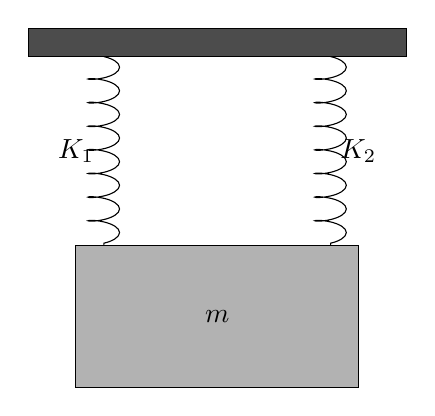
\begin{tikzpicture}[scale=1.2]

% Ceiling
\draw[fill=black!70] (-2,0) rectangle (2,0.3);

% Springs
\draw[decoration={coil,aspect=0.3,segment length=3mm,amplitude=2mm},decorate] (-1.2,0) -- (-1.2,-2);
\draw[decoration={coil,aspect=0.3,segment length=3mm,amplitude=2mm},decorate] (1.2,0) -- (1.2,-2);

% Labels for springs
\node[left] at (-1.2,-1) {$K_1$};
\node[right] at (1.2,-1) {$K_2$};

% Mass block
\draw[fill=black!30] (-1.5,-2) rectangle (1.5,-3.5);
\node at (0,-2.75) {$m$};

\end{tikzpicture}
\end{center}
\end{shaded}

La masa $m$ se mueve por la acción conjunta de los dos resortes. En particular,
por la segunda ley de Newton, 

\begin{equation*}
    R_1 + R_2 + G = ma
\end{equation*}

donde $R_1 = -k_1 \Delta y R_2 = -k_2 \Delta y$ y $G = -mg$. La distancia
$\Delta y$ es tal que la longitud de los resortes se duplica, i.e. la longitud
es de 0.5m. Esto significa que $\Delta y = -1 / 2 \text{m}$. Por lo tanto obtenemos 


\begin{align*}
    a 
    &= \frac{ -\left(-\frac{1}{2}\text{m}\right)50\text{N/m} - \left(
        -\frac{1}{2}\text{m}\right)100\text{N/m} - 2.5\text{kg} \cdot 9.8\text{m/s}^2
    }{2.5\text{kg}}\\ 
    &= \frac{25\text{N} + 50\text{N} - 24.5\text{N}}{2.5\text{kg}}\\ 
    &= \frac{50.5 \text{N}}{2.5\text{kg}} \\ 
    &=20.2\text{m/s}^2
\end{align*}

\pagebreak 

\begin{shaded}
    \textbf{(13)} Un resorte de constante elástica $k$ tiene un extremo fijo y
    el otro coincide con el punto $x_0$ cuando no está deformado. A este extremo
    se adhiere una masa $m$ que se desplaza hasta $x_1$, donde se la suelta. 
    $k = 8\text{N/m}, m = 2\text{kg}, x_0 = 40\text{cm}, x_1=55\text{cm}$.

    $(a)$ Determine las funciones de movimiento, velocidad y aceleración
    respecto al tiempo. 

    $(b)$ Determine el período, la frecuencia, las coordenadas extremas del
    movimiento, y el módulo de la velocidad de la masa $m$ en el punto de
    equilibrio.
\end{shaded}

$(a)$ Asumimos que no hay movimiento vertical. Sea $\omega = \sqrt{\frac{k}{m}}
$. Sabemos que

\begin{equation*}
    a(t) = -\omega^2 x(t), \qquad v(t) = \omega A \cos(\omega t + \phi), \qquad
    x(t) = x_0 + A \sin(\omega t + \phi)
\end{equation*}

con $x_0$ el punto de reposo. Las condiciones del problema establecen

\begin{equation*}
    x(t=0) = x_1 = 55\text{cm} = 0.55\text{m}, \qquad v(t=0) = 0
\end{equation*}

Sustituyendo $v(t = 0)$ por su evaluación, se tiene

\begin{equation*}
    \omega A \cos(\phi) = 0
\end{equation*}

Por def. sabemos que $\omega \neq 0$. Si $A$ fuera cero, entonces tendríamos
$x(t=0) = x_0$, lo cual es absurdo porque $x_0\neq x_1$. Por ende $A \neq 0$.
Pero entonces la ecuación anterior se satisface si y solo si $\cos(\phi) = 0$,
es decir si $\phi \in \left\{ \frac{\pi}{2}, -\frac{\pi}{2} \right\} $. Pero
restringimos $\phi$ a los reales positivos, obteniendo $\phi = \frac{\pi}{2}$.

Ahora tomemos $x(t = 0) = x_1$, y evaluamos la expresión izquierda sustituyendo
$\phi$ por $\frac{\pi}{2}$. Obtenemos

\begin{equation*}
    x_0 + A \sin(\phi) = x_1 \iff A = x_1 - x_0
\end{equation*}

Con esto lo hemos determinado todo. 

$(b)$ El periodo del movimiento oscilatorio harmónico se define como
$\frac{2\pi}{\omega}$. Pero 

\begin{equation*}
    \omega = \sqrt{\frac{k}{m}} = \sqrt{\frac{8\text{N/m}}{2\text{kg}}}  =
    \sqrt{4 \frac{1}{\text{s}^2}} = \frac{2}{\text{s}}
\end{equation*}

Por lo tanto, el período es 

\begin{equation*}
    \frac{2\pi}{\omega} = \frac{2\pi}{\frac{2}{\text{s}}} = \pi\text{s}
\end{equation*}

La frecuencia se define como la inversa del período, i.e.
$\frac{1}{\pi\text{s}} = \frac{1}{\pi}\text{Hz}$.

Las coordenadas máximas y mínimas son 

\begin{equation*}
    x_{\text{max}} = x_0 + A, \qquad x_{\text{min}} = x_0 - A
\end{equation*}

(lso casos en que el seno es uno y menos uno). Estos valores se pueden calcular
fácil. 

Observemos ahora que $x(t) = x_0$ si y solo si $A \sin(\omega t + \phi) = 0$,
i.e. si y solo si $\sin(\omega t + \phi) = 0$, i.e. si 
y solo si $\omega t + \phi = \pi$, lo cual se comple si y solo si 
$t = \frac{ \pi - \phi }{\omega}$

Pero $\phi = \frac{\pi}{2}$ y por lo tanto $\pi - \phi = \phi$. Luego $x(t) =
x_0$ si y solo si $t = \frac{\phi}{\omega}$. En dicho instante, la velocidad es 

\begin{align*}
    v\left(\frac{\phi}{\omega}\right) 
    &= \omega A \cos\left(\omega \cdot \frac{\phi}{\omega} +
    \phi\right)\\ 
    &= \omega A \cos(2\phi)  \\ 
    &=\omega A \cos(\pi) \\ 
    &=-\omega A
\end{align*}

Por lo tanto, el módulo de la velocidad en dicho instante es $\omega A$.

\pagebreak 

\begin{shaded}
    \textbf{(14)}. Sobre una superficie horizontal se fija un extremo de un resorte que tiene una longitud
natural de 0.5 m y cuya constante elástica es 400 N/m. Al otro extremo se une un
cuerpo de 2 kg de masa que se mueve de forma tal que describe una trayectoria
circular.
(a) Si el radio de la circunferencia es de 1 m, ¿Cual sera la velocidad del cuerpo?
(b) Si se duplica la velocidad, ¿Cual deberíaa ser el nuevo radio?
\end{shaded}


\begin{center}
    
\begin{tikzpicture}

\def\rr{3cm}
\def\nn{3}
\draw[thick, black] (0,0) circle (\rr);
\foreach \aa in {1,2,...,\nn}{
\begin{scope}[rotate={\aa*360/\nn+15}]
\draw [-latex, blue, ultra thick] (0:\rr) coordinate(dd\aa)--++(0,1.5cm)coordinate(aa\aa)node[right]{$\vv{v}$};
\draw [-latex, red, ultra thick] (0:\rr) --++(-1cm,0) node[right]{$\vv{a}$};
\draw [fill=black] (0:\rr) circle (0.1);
\end{scope}
\draw[ultra thick, gray,-latex] (-15:{\rr+0.5cm}) to [bend right=15] node[right]{$\omega$}(15:{\rr+0.5cm});
}

}

\draw (0,0) --(aa3)coordinate[pos=2](ff) -- (ff);
\draw (0,0) -- (dd3)coordinate[pos=2](ff) -- (ff);


\end{tikzpicture}
\end{center}

$(a)$ Nuestro sistema de coordenadas tendrá $\hat{i}$ antiparalelo a la
aceleración y $\hat{j}$ paralelo a la velocidad. Pues el movimiento es uniforme
sabemos que la aceleración tiene solo una componente centrípeta, i.e. 
$\vec{a} = a \hat{i}$ para algún $a < 0$. (Si $\hat{i}$ fuera paralelo en vez de
antiparalelo a la aceleración, sería $a > 0$.)

Por la segunda ley de Newton, la aceleración será la suma de las fuerzas
centrípetas dividida por la masa. Pero la única fuerza centrípeta es la del
resorte. Por lo tanto,

\begin{equation*}
    \vec{a} = \frac{\vec{R}}{m} \iff a = \frac{\left| \vec{R} \right| }{m} \iff
    a = -\frac{k}{m} \cdot \frac{1}{2}\text{m}
\end{equation*}

dado que la distancia entre el resorte y su punto de reposo es medio metro. Sin
embargo, el movimiento circular uniforme obedece la ley 

\begin{equation*}
    a = - \frac{v^2}{r}
\end{equation*}

(Si nuestro sistema de coordenadas tuviera $\hat{i}$ apuntanado hacia dentro,
i.e. centrípeto, sería $a = v^2 / r$). De los dos resultados hasta ahora
presentados, se sigue 

\begin{align*}
    \frac{v^2}{r} = \frac{k}{m} \cdot \frac{1}{2}\text{m}
    \iff 
    &\frac{v^2}{r} = \frac{400\text{N/m}}{2\text{kg}} \cdot \frac{1}{2}\text{m}\\ 
    \iff ~ ~ ~ 
    &\frac{v^2}{r} = 100 \text{m/s}^2
\end{align*}

Si $r = 1\text{m}$, entonces resulta 

\begin{equation*}
    v^2 = 100 (\text{m/s})^2 \iff v = 10\text{m/s}
\end{equation*}

lo cual resuelve el ejercicio.

$(b)$ Asumamos que se duplica la velocidad, i.e. que $v = 20\text{m/s}$. Notar
que ahora la tensión del resorte depende de un $r$ desconocido, y se obtiene

\begin{equation*}
    a = -\frac{k}{m} \cdot \Delta r
\end{equation*}

donde $\Delta r = r - \frac{1}{2}\text{m}$. Por ende,

\begin{align*}
    \frac{v^2}{r} = \frac{k\Delta r}{m}
    \iff 
    &\frac{400(\text{m/s})^2}{r} =  \Delta r \frac{400\text{N/m}}{2\text{kg}}\\
    \iff ~ ~ ~ 
    &\frac{1(\text{m/s})^2}{r} = \Delta r \frac{\text{N/m}}{2\text{kg}} \\ 
    \iff ~ ~ ~ 
    &\frac{1(\text{m/s})^2}{r} = \frac{ \Delta r }{2\text{s}^2}  \\ 
    \iff ~ ~ ~ 
    &\Delta r \cdot r = 2\text{m} \\ 
    \iff ~ ~ ~ 
    &r (r - \frac{1}{2}\text{m}) = 2\text{m} \\ 
    \iff ~ ~ ~ 
    &r^2 - \frac{r}{2}\text{m} - 2\text{m} = 0 
\end{align*}

Como $[r] = \text{m}$ las unidades son todas las mismas y simplemente nos
enfocamos en la función cuadrática $\varphi(x) = x^2 - \frac{x}{2} - 2$, con
raíces 

\begin{align*}
    x = \frac{0.5 \pm \sqrt{0.5^2 + 8}}{2} \iff x \in \left\{ 1.68614066163,
    -1.18614066163 \right\} 
\end{align*}

Pero obviamente el radio debe ser positivo. Por ende, nos quedamos con la raíz
positiva y concluimos $r \approx 1.686\text{m}$. 

\pagebreak 

\section{Guía 3}

\begin{shaded}
    \textbf{(1)} Considerá el diagrama siguiente: 
    \begin{center}
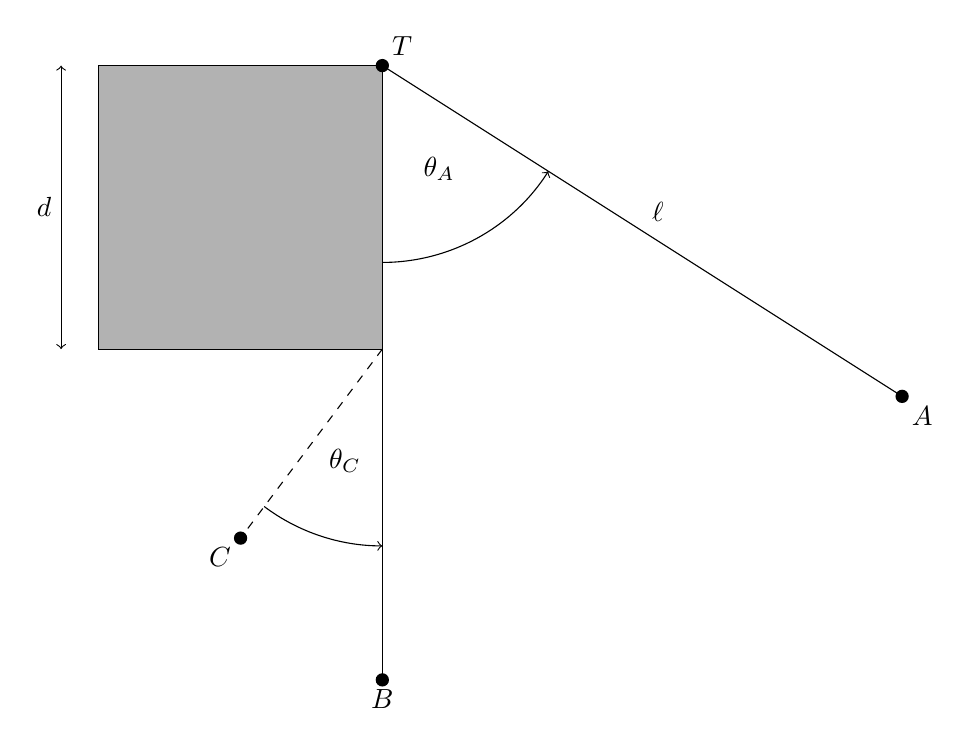
\begin{tikzpicture}[scale=1.2]

% Define points
\coordinate (T) at (0,0);          % top-right corner of square
\coordinate (B) at (0,-3);         % bottom-right corner of square
\coordinate (BL) at (-3,-3);       % bottom-left corner
\coordinate (TL) at (-3,0);        % top-left corner

% External points
\coordinate (A) at (5.5,-3.5);
\coordinate (C) at (-1.5,-5);
\coordinate (Bpt) at (0,-6.5);

% Draw square
\fill[gray!60] (T) -- (TL) -- (BL) -- (B) -- cycle;
\draw (T) -- (TL) -- (BL) -- (B) -- cycle;

% Dimension arrow for d
\draw[<->] (-3.4,0) -- (-3.4,-3) node[midway,left]{$d$};

% Rope TA
\draw (T) -- (A);
\draw (B) -- (Bpt);
\draw[dashed] (B) -- (C);

% Mark lengths
\path (T) -- (A) node[midway,above right]{$\ell$};

% Dots
\fill (T) circle (2pt) node[above right]{$T$};
\fill (A) circle (2pt) node[below right]{$A$};
\fill (Bpt) circle (2pt) node[below]{$B$};
\fill (C) circle (2pt) node[below left]{$C$};

% Angles
\pic[draw,->,angle radius=2.5cm,"$\theta_A$"] {angle = B--T--A};
\pic[draw,->,angle radius=2.5cm,"$\theta_C$"] {angle = C--B--Bpt};

\end{tikzpicture}
    \end{center}

    Una masa pequeña se coloca al final de la cuerda de largo $\ell =
    132\text{cm}$ y se suelte desde el reposo. Sabiendo que $\theta_A =
    \ang{5}, d = 66\text{cm}$, determinar: 

    $(a)$ La velocidad en el punto más bajo de la trayectoria. 

    $(b)$ El valor de $\theta_C$ para la máxima altura que alcanza la masa
    (punto C).

    $(c)$ La tensión de la cuerda en la posición $B$.

\end{shaded}

$(a)$ El sistema posee energía kinética (por el movimiento de la masa) y
potencial (por la gravedad, que es conservativa). Establezcamos nuestro sistema
de coordenadas con origen en el punto de reposo $B$ y crecimiento hacia arriba y
hacia la derecha. La energía potencial de la gravedad es $U = mg \Delta y$ con
$\Delta y$ la distancia vertical entre la masa (en un instante dado) y el punto
de reposo. Como el punto de reposo coincide con la coordenada $(0, 0)$, resulta
$U = mgy$.

Es fácil determina la altura de $A$ geométricamente. Si formamos un triángulo
rectángulo con $T$ y $A$, como se ve abajo en la figura,

    \begin{center}
\begin{tikzpicture}[scale=1.2]

% Define points
\coordinate (T) at (0,0);          % top-right corner of square
\coordinate (B) at (0,-3);         % bottom-right corner of square
\coordinate (BL) at (-3,-3);       % bottom-left corner
\coordinate (TL) at (-3,0);        % top-left corner

% External points
\coordinate (A) at (5.5,-3.5);
\coordinate (C) at (-1.5,-5);
\coordinate (Bpt) at (0,-6.5);
\coordinate (X) at (0, -3.5);        % top-left corner

% Rope TA
\draw (T) -- node[text midway, above]{$\ell$} (A);
\draw (T) -- node[text midway, left]{$\ell \cos \theta_A$} (X);
\draw (X) -- node[text midway, below]{$\ell \sin \theta_A$} (A);

\fill (X) circle (2pt) node[above right]{$X$};
\fill (T) circle (2pt) node[above right]{$T$};
\fill (A) circle (2pt) node[below right]{$A$};

\pic[draw,->,angle radius=2.5cm,"$\theta_A$"] {angle = B--T--A};

\end{tikzpicture}
\end{center}

obtenemos que la altura del punto $A$ es $\ell - \ell \cos \theta_A \approx
0.502\text{cm}$. 

Ahora bien, cuando la masa se encuentra en $A$ en el instante inicial, no hay
movimiento y por ende la energía es estrictamente potencial. Cuando la masa
cruza la posición de reposo, no hay energía potencial de la gravedad (pues la
altura es cero), y la energía es estrictamente cinética. Pero por preservación
de la energía, la energía en ambos instantes debe ser idéntica. Por lo tanto, 

\begin{align*}
    E_A = E_B \iff 
    &K_A + U_A = K_B + U_E \\ 
    \iff ~ ~ ~ 
    &0 + mg \Delta y = \frac{1}{2}mv_B^2 + 0\\ 
    \iff ~ ~ ~ 
    &2(9.8\text{m/s}^2)\left( \ell - \ell \cos \theta_A \right) = v^2_B \\ 
    \iff ~ ~ ~ 
    &9.84507709704 \cdot (\text{m/s}^2)\text{cm} = v^2_B \\ 
    \iff  ~ ~ ~
    &9.84507709704 \cdot (\text{m/s}^2)\text{cm} = v^2_B \\ 
    \iff  ~ ~ ~ 
    &0.09845077097 (\text{m/s}^2)\text{m} = v_B^2 \\ 
    \iff ~ ~ ~ 
    &v_B = 0.31376865836 \text{m/s}
\end{align*}

$(b)$ Se nos dice que la altura máxima que alcanza la masa es la de $C$, con lo
cual sabemos que en $C$ se detiene y la velocidad de la masa es cero ($v_C =
0$). Mismo razonamiento que antes: en $C$ la energía es estrictamente potencial,
pero en $B$ es estrictamente kinética. Por preservación de la energía,

\begin{equation*}
    E_B = E_C \iff 
    &\frac{1}{2}mv_B^2 = mg \Delta y
\end{equation*}

con $\Delta y$ la altura alcanzada en $C$. Pero conocemos $v_B$. Tomando la
aproximación $v_B \approx 0.314$, tenemos 

\begin{equation*}
    \Delta y = \frac{ \frac{1}{2}(0.314)^2(\text{m/s})^2 }{9.8\text{m/s}^2} =
    0.00503040816 \text{m} \approx 0.503\text{cm}
\end{equation*}

Para expresar lo que sabemos en un gráfico, tenemos:

\begin{center}
\begin{tikzpicture}[scale=1.2]

\coordinate (B) at (0,-3);         % bottom-right corner of square
\coordinate (C) at (-2.5,-5);
\coordinate (Bpt) at (0,-6.5);
\coordinate (Cpt) at (-2.5,-6.5);


% Rope TA
\draw (B) -- node[text midway, right=5pt]{$\ell - d$}(Bpt);
\draw[dashed] (B) -- node[text midway, left=5pt]{$\ell - d$} (C);
\draw[dashed] (C) -- node[text midway, left=5pt]{$\Delta y$} (Cpt);
\draw[dashed] (Cpt) -- node[text midway, below=5pt]{$\Delta x$} (Bpt);

% Dots
\fill (Bpt) circle (2pt) node[below=5pt]{$B$};
\fill (B) circle (2pt) node[above=pt]{$T$};
\fill (C) circle (2pt) node[below left=pt]{$C$};

% Angles
\pic[draw,->,angle radius=2.5cm,"$\theta_C$"] {angle = C--B--Bpt};

\end{tikzpicture}
\end{center}

donde $\Delta y, \ell - d$ son conocidos y $\Delta x$ solo es ilustrativo (no
nos importa.) Es claro que si formamos un triángulo rectángulo uniendo $C$ a la
línea $BT$, dicho triángulo satisface


\begin{center}
\begin{tikzpicture}[scale=2.2]

\coordinate (B) at (0,-3);         % bottom-right corner of square
\coordinate (C) at (-2.5,-5);
\coordinate (Cpt) at (-2.5,-6.5);
\coordinate (X) at (0,-5);


% Rope TA
\draw (B) -- node[text midway, left=5pt]{$\ell - d$} (C);
\draw (X) -- node[text midway, below=5pt]{$\Delta x = (\ell - d) \sin \theta_C$} (C);
\draw (B) -- node[text midway, right=5pt]{$\ell - d - \Delta y = ( \ell - d ) \cos
    \theta_C$} (X);

% Dots
\fill (X) circle (2pt) node[below=5pt]{$X$};
\fill (B) circle (2pt) node[above=5pt]{$T$};
\fill (C) circle (2pt) node[below=5pt left]{$C$};

% Angles
\pic[draw,->,angle radius=1.5cm,"$\theta_C$"] {angle = C--B--Bpt};

\end{tikzpicture}
\end{center}

Pero 

\begin{align*}
    \ell - d - \Delta y = (\ell - d)\cos \theta_C 
    \iff 
    &\cos \theta_C = \frac{\ell - d - \Delta y}{\ell - d} \\ 
    \iff ~ ~ ~ 
    &\cos \theta_C = 1 - \frac{\Delta y}{\ell - d} \\ 
    \iff  ~ ~ ~ 
    &\cos \theta_C = 1 - \frac{0.503\text{cm}}{132\text{cm} - 66\text{cm}} \\ 
    \iff ~ ~ ~ 
    &\cos \theta_C = 0.99237878787 \\ 
    \iff ~ ~ ~ 
    &\theta = 0.123538758
\end{align*}


$(c)$ Se nos pide la tensión de la cuerda en la posición de reposo. Consideremos
el movimiento del objeto como un movimiento circular. Las fuerzas en acción son
la gravedad (contraria al centro) y la tensión de la cuerda (centrípeta):

\begin{equation*}
    T - W = a_c m
\end{equation*}

con $a_c$ el conjunto de fuerzas con componente centrípeto, de acuerdo con la
segunda ley de Newton. Sin embargo, el movimiento circular siempre satisface
$a_c = v^2 / r$ con $r$ el radio de la circunferencia descrita por el
movimiento. Pero $r = \ell = 132\text{cm} = 1.32\text{m}$. Por lo tanto, 

\begin{equation*}
    T - W = \frac{v^2 m}{\ell}
\end{equation*}

La velocidad en el punto $B$ ya la conocemos. Sustituyendo y sumando $W = mg$ a
ambos lados, con un poco de álgebra se obtiene

\begin{equation*}
    T  = m \left( \frac{0.314^2}{132} \text{m/s}^2 + 9.8 \text{m/s}^2  \right) =
    m(9.80074693939 \text{m/s}^2)
\end{equation*}

Como $[m] = \text{kg}$, se tiene correctamente $[T] = \text{N}$.

\pagebreak 

\begin{shaded}
    \textbf{(2)} Un bloque de 20kg es empujado sobre una superficie horizontal
    por medio de una fuerza $\vec{F}$ que forma un ángulo $\theta$ con la misma.
    La magnitud de la fuerza cuando la masa está en la posición $x$ es 
    $\left| \vec{F}(x) \right| = 6x \text{N}$. 

    $(a)$ Calcular el trabajo realizado por la fuerza en el intervalo $x \in
    [10\text{m}, 20 \text{m}]$.

    $(b)$ Calcule la energía cinética del cuerpo en la posición final para
    $\mu_d = 0, \mu_d = 0.05$, asumiendo que se parte del reposo.

\end{shaded}

$(a)$ Recordemos que por def. el trabajo realizado por una fuerza $\vec{F}$ al
obrar un desplazamiento $\vec{\Delta r}$ es el producto punto entre ambos:

\begin{equation*}
    W_F = \vec{F} \cdot \vec{\Delta r} = F \Delta r \cdot \cos \theta
\end{equation*}

con $\theta$ el ángulo entre ambos. En nuestro caso, la magnitud de $\vec{F}$ es
variable (no así el ángulo $\theta$), y por lo tanto 

\begin{align*}
    W_F 
    &= \int_{10}^{20} \left| \vec{F}(x) \right| \cos \theta ~ dx\\ 
    &= 6\text{N} \cos \theta \int_{10}^{20} x ~ dx\\ 
    &= 6\text{N} \cos \theta \left[ \frac{x^2}{2} \right]_{10}^{20} \\ 
    &=6\text{N}\cos\theta \left( 150\text{m} \right) \\ 
    &=900 \cos \theta \text{Nm} \\ 
    &= 900 \cos\theta \text{ J}
\end{align*}

$(b)$


\small
\begin{quote}

Entiendo que el ejercicio pide desde $x = 0\text{m}$ hasta $x=20\text{m}$. De
cualquier modo, el procedimeinto es esl mismo para un desplazamiento desde 
$x = 10\text{m}$ hasta $x=20$m.

\end{quote}
\normalsize


Recordemos que $W = \Delta K$. Pero la energía cinética en el instante
cero es nula y por lo tanto resulta $W = K_f$. Es decir, la energía cinética en
el instante final es el trabajo neto de las fuerzas a lo largo de todo el
recorrido: 

\begin{equation*}
    W = W_F + W_R
\end{equation*}

con $W_R$ el trabajo realizado por la fuerza de rozamiento. El ángulo entre la
fuerza de rozamiento y la dirección del movimiento es de 180 grados, pues se
oponen, y por ende su coseno es $-1$. Es decir que la fuerza de rozamiento hace un trabajo
negativo:

\begin{align*}
    W_R 
    &= -\left| \vec{R} \right| \Delta x \\ 
    &= - \mu\left| \vec{N} \right| 20\text{m} \\ 
    &= - \mu mg 20\text{m} \\ 
    &= - \mu (20 \cdot 9.8 \cdot 20) (\text{kg} \cdot \text{m/s}^2 \cdot
    \text{m}) \\ 
    &= -\mu 3920 \text{ J}
\end{align*}

Por el mismo razonamiento que antes, 

\begin{equation*}
    W_F = 6\text{N} \cos \theta\int_{0}^{20} x ~ dx = 1200 \cos \theta \text{ J}
\end{equation*}

Por lo tanto, 

\begin{equation*}
    W = 1200 \cos \theta \text{ J} - \mu 3920 \text{ J}
\end{equation*}

\pagebreak 

\section{P4}

\begin{shaded}
    \textbf{(1)} Determinar el campo eléctrico en un punto a 12cm de una carga
    de $-4 \times 10^{-9}$C. ¿Cuál sería el vector fuerza $\vec{F}$ que
    experimentaría un electrón situado en dicha posición?
\end{shaded}

$(a)$ Recordemos que el campo eléctrico no es más que la fuerza que experimentaría una
carga positiva y unitaria a una distancia $d$ de una carga de referencia. Es
decir, es la fuerza electroestática \textit{normalizada}. Más formalmente, dada
una carga de referencia $Q$ y una carga $q$,

\begin{equation}
    \vec{E} = \frac{ \vec{F}_e }{q} = \frac{1}{4\pi \epsilon_0}
    \frac{Q}{r^2} ~ \hat{r}
\end{equation}

con $\hat{r}$ un vector unitario de dirección (de $Q$ a $q$). En este caso, $r =
12\text{cm} = 0.12\text{m}$. Tomando $\kappa = 1 / 4\pi\epsilon_0$:

\begin{equation}
    \vec{E} 
    &= \kappa  \frac{-4 \times 10^{-9} C}{0.0144 \text{m}^2} ~ \hat{r}
\end{equation}

Con $\epsilon_0 = 8.854187817\times 10^{-12} \text{F/m}$, se obtiene la
aproximación 

\begin{equation}
    \kappa \approx 8.99 \times 10^{9} \text{N} \cdot \frac{ \text{m}^2
    }{\text{C}^2}
\end{equation}

Usaré 9 en vez de 8.99. La ecuación $(2)$, separando por un lado los factores
numéricos y por otro los factores unidad, resulta entonces

\begin{align*}
    \vec{E} 
    &= ( 8.99 \times 10^{9} ) \cdot \frac{-4 \times 10^{-9}}{0.0144} ~ \times 
    \left( \text{N} \cdot \frac{\text{m}^2}{\text{C}^2} \right)\left(
    \frac{\text{C}}{\text{m}^2} \right)  \times \hat{r} \\
    &= \frac{9}{3.6} \times ( -10^{3} ) \text{N/C} ~ \hat{r}\\ 
    &=-2497.222 \text{N/C} ~ \hat{r}
\end{align*}

$(b)$ La carga de un electrón es $-1.602 \times 10^{-19}\text{C}$. La fuerza que
experimenta una carga $q$ en un campo magnético $\vec{E}$ es $\vec{F} =
q\vec{E}$. Por lo tanto, el electrón experimenta la fuerza 

\begin{align*}
    \vec{F} 
    &= \left( -1.602 \times 10^{-19} \text{C} \right) \times -2497.222
    \text{N/C} ~ \vec{r} \\ 
    &= 4000.549644 \times 10^{-19} \text{N} ~ \hat{r}
\end{align*}

Notemos que la fuerza es positiva, lo cual significa que el electrón es repelido
por la carga de referencia que genera el campo magnético. Esto tiene sentido,
porque tanto la carga del electrón como la carga de referencia $Q$ son negativas.

\pagebreak 

\begin{shaded}
    \textbf{(2)}
\end{shaded}

(a) Recordemos que al calcular una fuerza electroestática, la constanta $\kappa
= 1 / 4\pi \epsilon_0$ tiene unidades N (m$^2$/C$^2$), y al multiplicarla por el
producto de las cargas sobre la distancia al cuadrado, solo nos queda N:

\begin{equation*}
    \left[ \text{N} \frac{\text{m}^2}{\text{C}^2} \right] \left[
    \frac{\text{C}^2}{\text{m}^2} \right] = \left[ \text{N} \right] 
\end{equation*}

Por lo tanto, nos ahorraremos este cálculo de unidades y de ahora en adelante
escribiremos directamente la fuerza en Newton, obviando las otras unidades.
Usando la aproximación $\kappa = 8.99 \times 10^9$, con $r^2 = 0.25$ (metros al
cuadrado), 

\begin{align*}
    F_{12} &= 
    \kappa \frac{ 2 \times 10^{-12}}{0.25} ~ \hat{r}  ~ \text{N} = 0.07192 ~ \text{N}& \left\{
\text{Atractiva} \right\} \\ 
    F_{13} &= \kappa \frac{3 \times 10^{-12} }{0.25} \text{N} = 0.10788  ~ \text{N}&\left\{ \text{Repulsiva} \right\} \\ 
    F_{23} &= \kappa \frac{ 6 \times 10^{-12} }{0.25} \text{N} = 0.21576  ~ \text{N} &\left\{ \text{Atractiva} \right\} 
\end{align*}

Ahora bien, cada carga está en el campo eléctrico de las otras dos, i.e. es
afectada por ambas. Por lo tanto, la fuerza que experimentada por cada carga es 

\begin{align*}
    F_1 &= F_{12}\hat{i} - \hat{i}F_{13} = \hat{i}(0.07192 -
    0.10788)\text{N} = -0.03596\text{N} ~ \hat{i} \\ 
    F_2 &= -\hat{i} F_{12} + \hat{i} F_{13} = \hat{i}(-0.07192 + 0.10788)\text{N}
    = 0.03596\text{N} ~  \hat{i}\\ 
    F_3 &= -\hat{i}F_{23} + \hat{i}F_{13} = \hat{i}(-0.21576 + 0.10788)\text{N}
    = -0.10788\text{N} ~ \hat{i}
\end{align*}

$(c)$ 

\begin{align*}
    V_1 = \kappa \left( \frac{q_2}{0.5} + \frac{q_3}{1} \right)  \\ 
    V_2 = \kappa \left( \frac{q_1}{0.5} + \frac{q_3}{1} \right)  \\ 
    V_3 = \kappa \left( \frac{q_1}{1} + \frac{q_2}{0.5} \right)  
\end{align*}

\pagebreak 

\textbf{(3)} Consideremos solo la bola derecha. Tenemos que 

\begin{equation*}
    \vec{T} + \vec{E} + \vec{P} = 0
\end{equation*}

Si notamos que $\vec{E}$ no tiene componente vertical y $\vec{P}$ no tiene
componente horizontal, esto implica que

\begin{align*}
    (T_x + E)\hat{i} + (T_y + P) \hat{j} = 0
\end{align*}

o bien 

\begin{equation}
    \begin{cases}
        T_x = -E \\ 
        T_y = -P
    \end{cases}
\end{equation}

Ahora bien, es fácil observar geométricamente que 

\begin{equation}
    \vec{T} = T_x \hat{i} + T_y \hat{j} = T \sin \theta \hat{i} + T \cos \theta
    \hat{j}
\end{equation}

Expresado de una forma más bonita:

\begin{equation}
    \begin{cases}
        T_x = T \sin \theta \\ 
        T_y = T \cos \theta
    \end{cases}
\end{equation}

Como $T_y = -P$ por (4), y $P = -mg$,

$$T_y = mg = 30\text{g} \cdot 9.8 \frac{m}{s^2} = 0.1943 \text{N}$$

La segunda ecuación del sistema $(6)$ nos da $T = T_y /\cos \theta$ y por lo
tanto obtenemos 

\begin{align*}
    T &= \frac{0.1943 \text{N}}{\cos \ang{5}} = \frac{0.1943
    \text{N}}{0.99619469809}  = 0.19504219443\text{N}
\end{align*}

Podemos usar esto para despejar $T_x$ en $(6)$: 

\begin{equation*}
    T_x = 0.19504219443\text{N} ~ \sin \theta = 0.01699904732
\end{equation*}

Por (4), sabemos que $T_x = -E$. Por lo tanto, 

\begin{equation}
    E = -0.01699904732\text{N}
\end{equation}





















\end{document}



